The second task requires us to design a more complex environment and subsequently re-running both the Value Iteration and Policy Iteration algorithms on it. 

\subsection{Approach}
To assess the impact of increasing the number of states and the complexity of the maze on convergence, we focus on two key factors: maze size and state distribution. First, we expand the grid from 6×6 to 10×10, significantly increasing the number of states, which enlarges the state space and potentially extends convergence times. Second, we modify the distribution of tile types, reducing the number of high-reward states while increasing obstacles and penalty tiles. Additionally, since the tile positions are randomly assigned, the environment lacks a predefined "end goal" (like in the 6x6 maze in Part 1), making the learning process more challenging as there is no immediate attractor for value propagation. \vspace{10pt}

\noindent In Part 1, the original maze consists of \textbf{Brown (0.14)}, \textbf{White (0.55)}, \textbf{Wall (0.14)}, and \textbf{Green (0.17)} tiles. To introduce greater complexity in Part 2, we modify these proportions to \textbf{Brown (0.35)}, \textbf{White (0.30)}, \textbf{Wall (0.30)}, and \textbf{Green (0.05)} in a 10×10 maze. This shift increases penalties and obstacles, restricting available paths and making convergence more challenging. We hypothesize that these changes will lead to longer iteration times and potentially slower policy stabilization.

\subsection{Implementation}
\begin{figure}[H]
    \centering
    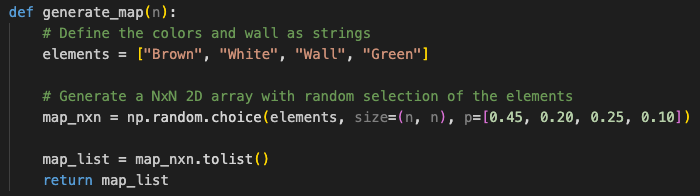
\includegraphics[width=0.8\textwidth]{images/generate.png}
    \caption{Function to Generate an \(N \times N\) Maze}
    \label{fig:10x10_maze_function}
\end{figure}

\subsection{How does the number of states and the complexity of the environment affect convergence?}

We observed an interesting trend in the convergence behavior of Value Iteration and Policy Iteration. For Value Iteration, the number of iterations required to reach convergence remained consistent at approximately 690 iterations, regardless of the environment's complexity. In contrast, Policy Iteration exhibited significantly slower convergence, exceeding 100,000 iterations without achieving convergence. Even when increasing the value of $\theta$ (the convergence threshold) to 0.01 and 0.05, the number of iterations for Policy Iteration remained above 100,000, indicating that the algorithm struggled to handle the increased complexity. \vspace{10pt}

\noindent This behavior is expected, as environments with a larger number of states and greater complexity inherently require more iterations to converge. The need to evaluate and update a larger state space naturally increases the computational burden, particularly for algorithms like Policy Iteration, which involve policy evaluation and improvement steps that can become computationally expensive in complex environments.

\subsection{How complex can you make the environment and still be able to learn the right policy?}

In theory, given sufficient computational resources, algorithms like Value Iteration and Policy Iteration can learn the optimal policy even in highly complex environments, such as an NxN grid where N is extremely large. However, as the environment grows in complexity, the feasibility of using these methods diminishes due to the exponential increase in computational requirements. While these algorithms are guaranteed to converge to the optimal policy under ideal conditions, their practical application becomes infeasible for very large or complex environments. In such cases, alternative approaches—such as approximate dynamic programming, reinforcement learning, or heuristic methods—should be explored to achieve a balance between computational efficiency and policy accuracy.
